%% CPT-Symmetric Universe -- Beamer Presentation
%% Wei-Ning Deng, Theoretical Cosmology Seminar, 17 Feb 2026
%% Compile with: pdflatex (or xelatex for better font support)

\documentclass[aspectratio=169]{beamer}

%% ---------------------------------------------------------------
%%  Packages
%% ---------------------------------------------------------------
\usepackage{amsmath,amssymb,amsfonts}
\usepackage{graphicx}
\usepackage{multimedia}
\usepackage{xcolor}
\usepackage{tikz}
\usetikzlibrary{arrows.meta, positioning, shapes.geometric}
\usepackage{hyperref}
\usepackage{booktabs}
\usepackage{multicol}
\usepackage{slashed}

%% ---------------------------------------------------------------
%%  Theme
%% ---------------------------------------------------------------
\usetheme{default}
\usecolortheme{default}
\usefonttheme{professionalfonts}

% Clean, minimal style
\setbeamertemplate{navigation symbols}{}
\setbeamercolor{footline bar}{bg=cptblue!15, fg=darkgray}
\setbeamertemplate{footline}{%
  \leavevmode%
  \begin{beamercolorbox}[wd=\paperwidth,ht=2.25ex,dp=1ex]{footline bar}%
    \hspace{1em}%
    \usebeamerfont{author in head/foot}$\langle$\texttt{wnd22@cam.ac.uk}$\rangle$%
    \hfill
    \texttt{weiningdeng.com}%
    \hfill
    \insertframenumber{} / \inserttotalframenumber%
    \hspace{1em}%
  \end{beamercolorbox}%
}
\setbeamertemplate{itemize items}[circle]

% Colour palette
\definecolor{cptblue}{RGB}{0,112,192}
\definecolor{cptyellow}{RGB}{255,215,0}
\definecolor{cptred}{RGB}{192,0,0}
\definecolor{cptgreen}{RGB}{0,150,60}
\definecolor{darkgray}{RGB}{50,50,50}

\setbeamercolor{frametitle}{fg=darkgray}
\setbeamercolor{title}{fg=darkgray}
\setbeamercolor{structure}{fg=cptblue}

%% ---------------------------------------------------------------
%%  Title info
%% ---------------------------------------------------------------
\title{\textbf{The CPT-Symmetric Universe:}\\
       From Quantized Curvature to K\"{a}hler-Dirac Fermions}
\author{Wei-Ning Deng \\ \small\texttt{wnd22@cam.ac.uk}}
\institute{Theoretical Particle Physics \& Cosmology Group\\
           King's College London}
\date{2026}

%% ---------------------------------------------------------------
%%  Helper commands
%% ---------------------------------------------------------------
\newcommand{\arxiv}[1]{[arXiv:\,#1]}
\newcommand{\Red}[1]{{\color{cptred}#1}}
\newcommand{\Blue}[1]{{\color{cptblue}#1}}
\newcommand{\Green}[1]{{\color{cptgreen}#1}}
\newcommand{\Yellow}[1]{{\color{cptyellow}#1}}

\newcommand{\figpath}{../figures/}   % all figures live here

%%================================================================
\begin{document}
%%================================================================

%% ---- Title slide -----------------------------------------------
\begin{frame}[plain]
  \begin{tikzpicture}[remember picture, overlay]
    \node[at=(current page.center)] {
      \includegraphics[width=\paperwidth,height=\paperheight,
                       keepaspectratio=false]{\figpath CPT_periodic.png}
    };
    \fill[white, opacity=0.0] (current page.south west) rectangle (current page.north east);
    %% Title at the top
    \node[anchor=north, text=white, align=center, yshift=-0.3cm] at (current page.north) {
      \parbox{0.9\paperwidth}{\centering
        {\Large\textbf{The CPT-Symmetric Universe:}}\\[0.3em]
        {\large From Quantized Curvature to K\"{a}hler-Dirac Fermions}
      }
    };
    %% Name and seminar info at the bottom
    \node[anchor=south, text=white, align=center, yshift=0.3cm] at (current page.south) {
      \parbox{0.9\paperwidth}{\centering
        {\normalsize Wei-Ning Deng, University of Cambridge (\texttt{wnd22@cam.ac.uk})}\\[0.2em]
        {\small TPPC Seminar, King's College London (2026)}
      }
    };
  \end{tikzpicture}
\end{frame}

%% ---- Outline ---------------------------------------------------
\begin{frame}{Outline}
  \textbf{Part 1: Introduction -- CPT-symmetric universe}\\[0.5em]
  Part 2: Theoretical prediction of spatial curvature
  \small (PRD\,110,\,103528;\; PRD\,113,\,023546)\\[0.5em]
  Part 3: K\"{a}hler-Dirac fermions -- Physical foundation of CPT
  \small (arXiv:2511.11548)\\[0.5em]
  Future directions: Lattice KD,\; Composite Higgs,\; Quadratic gravity

  \vspace{0.4cm}
  \begin{columns}[c]
    \column{0.45\textwidth}\centering
      \includegraphics[height=3.8cm]{\figpath wh260.jpg}\\
      {\small Will Handley (University of Cambridge)\\
       \texttt{wh260@cam.ac.uk}}
    \column{0.45\textwidth}\centering
      \includegraphics[height=3.8cm]{\figpath lboyle3.jpg}\\
      {\small Latham Boyle (University of Edinburgh)\\
       \texttt{Latham.Boyle@ed.ac.uk}}
  \end{columns}
\end{frame}

%%================================================================
%%  PART 1 -- Introduction: CPT-Symmetric Universe
%%================================================================
\begin{frame}{Outline}
  \textbf{\Blue{Part 1: Introduction -- CPT-symmetric universe}}\\[0.5em]
  Part 2: Theoretical prediction of spatial curvature
  \small (PRD\,110,\,103528;\; PRD\,113,\,023546)\\[0.5em]
  Part 3: K\"{a}hler-Dirac fermions -- Physical foundation of CPT
  \small (arXiv:2511.11548)\\[0.5em]
  Future directions: Lattice KD,\; Composite Higgs,\; Quadratic gravity

  \vspace{0.4cm}
  \begin{columns}[c]
    \column{0.45\textwidth}\centering
      \includegraphics[height=3.8cm]{\figpath wh260.jpg}\\
      {\small Will Handley (University of Cambridge)\\
       \texttt{wh260@cam.ac.uk}}
    \column{0.45\textwidth}\centering
      \includegraphics[height=3.8cm]{\figpath lboyle3.jpg}\\
      {\small Latham Boyle (University of Edinburgh)\\
       \texttt{Latham.Boyle@ed.ac.uk}}
  \end{columns}
\end{frame}

%% ------------------------------------------------------------------
%%  P1-1  Theoretical and Observational Challenges
%% ------------------------------------------------------------------
\begin{frame}{Theoretical and observational challenges}
  \begin{columns}[c]
    \column{0.55\textwidth}
      \begin{enumerate}
        \item \textbf{Problems in cosmology:}\\
              Cosmological constant problem, nature of DM,
              origin of matter--antimatter asymmetry
        \item \textbf{Problems in particle physics:}\\
              Hierarchy problem, strong CP problem,
              origin of 3 fermion generations
        \item \textbf{Observational challenges:}\\
              BICEP/Keck \arxiv{2203.16556}: tight constraint
              on inflationary B-modes ($r < 0.036$)
        \item \textbf{No prediction for $\Omega_K$:}\\
              Treated as a free parameter -- but Planck 2018
              shows a $2\sigma$ preference for $\Omega_K < 0$
      \end{enumerate}
    \column{0.45\textwidth}
      \includegraphics[width=\textwidth]{\figpath r_vs_ns_bk18.pdf}
  \end{columns}
\end{frame}

%% ------------------------------------------------------------------
%%  P1-2  CPT-symmetric universe
%% ------------------------------------------------------------------
\begin{frame}{CPT-symmetric universe}
  \begin{center}
    \includegraphics[width=\textwidth]{\figpath CPT-symmetric_universe.png}
  \end{center}
  \vspace{-0.5em}
\end{frame}

%% ------------------------------------------------------------------
%%  P1-3  CMB acoustic peaks: Neumann BC as evidence for a temporal mirror
%% ------------------------------------------------------------------
\begin{frame}{CMB acoustic peaks: direct evidence for a temporal mirror}
  \begin{columns}[c]
    \column{0.55\textwidth}
      \includegraphics[width=\textwidth]{\figpath A15_TT.png}\\
      % {\scriptsize Planck 2018 CMB TT power spectrum -- acoustic oscillations}
    \column{0.4\textwidth}
      \includegraphics[width=\textwidth]{\figpath CPT_periodic.png}\\[0.3em]
      % {\scriptsize Perturbations with Neumann (reflecting) BC at $\eta=0$}
  \end{columns}
  \begin{block}{}
    \footnotesize
    The \textbf{ringing pattern} in the CMB TT (and TE) power spectra is direct evidence
    that primordial density perturbations obeyed a
    \Blue{\textbf{reflecting (Neumann) BC}} at the start of the radiation era:
    \[
      \dot\Phi\big|_{\eta=0} = 0
      \quad\Longleftrightarrow\quad
      \text{Big Bang acts as a \textbf{temporal mirror}}
    \]
    If radiation era was \emph{not} preceded by inflation, it's
    \Red{direct obs. evidence} that BB is a temporal mirror.
  \end{block}
\end{frame}

%% ------------------------------------------------------------------
%%  P1-5  CPT solves lots of problems
%% ------------------------------------------------------------------
\begin{frame}{CPT-symmetry universe can solve lots of problems}
  \small (Proposed by Latham Boyle and Neil Turok)
  \vspace{0.4em}

  \begin{center}
  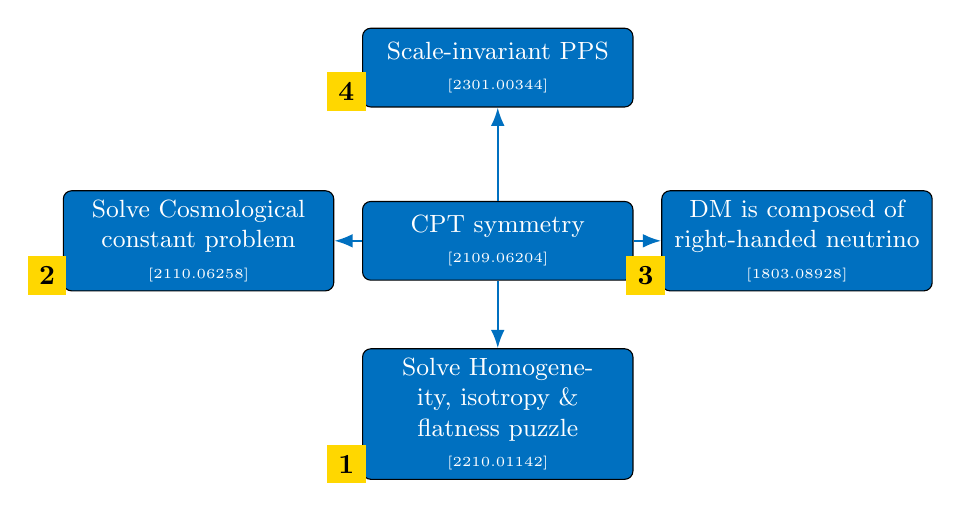
\begin{tikzpicture}[
      box/.style={draw, fill=cptblue, text=white, rounded corners=3pt,
                  text width=3.2cm, align=center, minimum height=1.0cm,
                  font=\small},
      arr/.style={-Latex, thick, cptblue},
      num/.style={fill=cptyellow, text=black, font=\bfseries,
                  inner sep=2pt, minimum size=14pt}
    ]
    \node[box] (cpt) at (0,0) {CPT symmetry \\ {\tiny [2109.06204]}};
    \node[box] (flat) at (0,-2.2) {Solve Homogeneity, isotropy \& flatness puzzle \\ {\tiny [2210.01142]}};
    \node[box] (cc)   at (-3.8,0) {Solve Cosmological constant problem \\ {\tiny [2110.06258]}};
    \node[box] (dm)   at ( 3.8,0) {DM is composed of right-handed neutrino \\ {\tiny [1803.08928]}};
    \node[box] (pps)  at (0, 2.2) {Scale-invariant PPS \\ {\tiny [2301.00344]}};

    \draw[arr] (cpt) -- (flat);
    \draw[arr] (cpt) -- (cc);
    \draw[arr] (cpt) -- (dm);
    \draw[arr] (cpt) -- (pps);

    \node[num] at ([shift={(-0.2,0.2)}]flat.south west) {1};
    \node[num] at ([shift={(-0.2,0.2)}]cc.south west)   {2};
    \node[num] at ([shift={(-0.2,0.2)}]dm.south west)   {3};
    \node[num] at ([shift={(-0.2,0.2)}]pps.south west)  {4};
  \end{tikzpicture}
  \end{center}
\end{frame}



%% ------------------------------------------------------------------
%%  P1-5  Analytic solution of Friedmann equation
%% ------------------------------------------------------------------
\begin{frame}{Analytic solution of Friedmann equation in conformal time}
  \begin{columns}[c]
    \column{0.5\textwidth}
      \begin{block}{}
        \vspace{-2em}
        \textbf{Metric:}
        \[
          ds^2 = a(t)^2\!\left(-dt^2 + \gamma_{ij}\,dx^i dx^j\right)
        \]
        \vspace{-0.5em}
        \textbf{Friedmann equation} (Planck units):
        \[
          3\dot{a}^2 = \underbrace{r}_{\text{rad}}
                     + \underbrace{\mu a}_{\text{matter}}
                     - \underbrace{3\kappa a^2}_{\text{curvature}}
                     + \underbrace{\lambda a^4}_{\Lambda}
        \]
        \vspace{0.2em}
        \textit{General solution (Jacobi elliptic function):}\\
        \textit{$a(t)$ is doubly periodic in the complex $t$-plane.}\\
        {\small The imaginary time period and the action computed over a period
         determine $T_H$ and the gravitational entropy $S_g$.
        (thermodynamics selects the most probable universe).}  
        \vspace{0.1em}
      \end{block}
    \column{0.5\textwidth}
      \includegraphics[height=3cm,keepaspectratio]{\figpath ScaleFactorFigv2.png}\\[0.2em]
      \begin{center}
        \includegraphics[height=3.8cm,keepaspectratio]{\figpath TorusFig2.png}\\
        {\scriptsize Euclidean torus: imaginary-time instanton}
      \end{center}
  \end{columns}
\end{frame}


%% ------------------------------------------------------------------
%%  flat universe most probable
%% ------------------------------------------------------------------
\begin{frame}{Flat, isotropic, homogeneous universe is most probable}
  \begin{center}
    \includegraphics[height=7cm,keepaspectratio]{\figpath Homo_iso_flat_universe.png}
  \end{center}
\end{frame}


%% ------------------------------------------------------------------
%%  P1-11a  Gravitational UV fixed points (arXiv:2509.09346)
%% ------------------------------------------------------------------
\begin{frame}{Gravitational UV fixed points}
  \begin{columns}[T]
    \column{0.57\textwidth}
      {\small
      \textbf{Problem:} coupling QFT to gravity $\Rightarrow$ UV divergences in
      $\langle T_{\mu\nu}\rangle$, implying wildly curved spacetime on short scales.}

      \vspace{0.3em}
      {\small \textbf{ERGE approach:} identify UV fixed points where
      \emph{all} gravitational $\beta$-functions vanish.\\
      {\scriptsize Boyle, Turok, Vaibhav, arXiv:2509.09346}}

      \vspace{0.3em}
      {\small \textbf{Beta functions:}
      \begin{align*}
        &\beta_{\Lambda/G} \propto n_0 - 2n_{1/2} + 2n_1 + 2n'_0 = 0\\[1pt]
        &\beta_i\, \text{(four-deriv.\ terms)} = 0,\quad i=1,2,3,4
      \end{align*}}

      {\small \textbf{All $\beta$-functions vanish iff:}}
      \begin{equation*}
        \boxed{n_{1/2} = 4n_1,\quad n'_0 = 3n_1,\quad n_0 = 0}
      \end{equation*}

    \column{0.40\textwidth}
      {\small \textbf{Conformally coupled fields:}
      \begin{itemize}
        \item $n_1$: gauge fields
        \item $n_{1/2}$: Weyl/Majorana fermions
        \item $n_0$: Klein-Gordon scalars\\
              {\scriptsize standard 2-derivative}
        \item $n'_0$: Fradkin-Tseytlin (FT) scalars\\
              {\scriptsize 4-derivative conformally coupled}
      \end{itemize}}

      \vspace{0.em}
      {\small \textbf{At the fixed point:}
      \begin{itemize}
        \item $G(k)\sim k^{-2}$ in UV (``softening'')
        \item $\langle T_{\mu\nu}\rangle$ and all $\langle TT\rangle$ UV-finite
        \item \Red{Cosmological constant problem solved}
      \end{itemize}}
  \end{columns}
\end{frame}

%% ------------------------------------------------------------------
%%  P1-11b  Standard Model at the gravitational fixed point
%% ------------------------------------------------------------------
\begin{frame}{Standard Model at the gravitational fixed point}
  \begin{columns}[T]
    \column{0.56\textwidth}
      SM gauge group $SU(3)\!\times\!SU(2)\!\times\!U(1)$:
      $n_1 = 8+3+1 = 12$ gauge fields\\[0.5em]

      \begin{tabular}{lcc}
        \hline\\[-0.8em]
        & Required & SM (incl.\ $\nu_R$) \\[0.2em]
        \hline\\[-0.7em]
        Fermions $n_{1/2}$ & $4\times 12=48$ & $3\times 16=\mathbf{48}$ \checkmark\\[0.2em]
        KG scalars $n_0$   & $0$             & Higgs $\to$ composite\\[0.2em]
        FT scalars $n'_0$  & $3\times 12=36$ & $0$ \quad (to predict!)\\[0.2em]
        \hline
      \end{tabular}\\[0.6em]

      \textbf{Predictions:}
      \begin{enumerate}\small
        \item \textbf{3 generations + $\nu_R$:} $n_{1/2}\!=\!48$
              requires right-handed neutrinos
        \item \textbf{Composite Higgs:} $n_0\!=\!0$ forbids fundamental
              KG scalars
        \item \textbf{36 FT (dim-0) scalars} also generate scale-invariant
              primordial spectrum!
      \end{enumerate}
    \column{0.41\textwidth}
      \includegraphics[width=\textwidth]{\figpath SM_particles.png}\\[0.4em]
      {\small IR: positive $G$ + arbitrarily small $\Lambda$\\[0.3em]
      {\scriptsize arXiv:2509.09346}}
  \end{columns}
\end{frame}

%% ------------------------------------------------------------------
%%  P1-12  Extended SM: RH neutrinos + Dim-0 scalars
%% ------------------------------------------------------------------
\begin{frame}{Extended Standard Model: 3 $\nu_R$ + 36 dim-0 scalars}
  \begin{center}
    \includegraphics[height=7cm]{\figpath SM_particles_dim0_RHnu.png}
  \end{center}
\end{frame}



%% ------------------------------------------------------------------
%%  P1-7  Right-handed neutrino as dark matter (expanded for KCL)
%% ------------------------------------------------------------------
\begin{frame}{Right-handed neutrino as dark matter}
  \begin{columns}[T]
    \column{0.52\textwidth}
      \textbf{CPT-symmetric universe predicts:}
      \begin{itemize}
        \item $\mathbb{Z}_2$ symmetry stabilises \emph{one} $\nu_R$
              $\Rightarrow$ \textbf{lightest neutrino is massless}
        \item The stable $\nu_R$ is produced via metric time-dependence
              when $H\sim M$ (analogous to Hawking radiation)
        \item $\nu_R$ dark matter mass:
              $M_{\nu_R}\approx 5\times10^8\,\text{GeV}$
              {\scriptsize \arxiv{1803.08928}}
        \item \Red{Falsifiable:} lightest $\nu$ massless
              $\Rightarrow$ normal hierarchy,
              $\sum m_\nu \approx 0.06\,\text{eV}$\\
              \Green{EUCLID, CMB-S4, LSST will test this}
      \end{itemize}
    \column{0.44\textwidth}
      \includegraphics[height=2.7cm,keepaspectratio]{\figpath CPT-symmetric_universe.png}\\[0.2em]
      \includegraphics[height=3.0cm,keepaspectratio]{\figpath mnu_constraints.pdf}\\
      {\scriptsize sum neutrino mass (eBOSS 2007.08991)}
  \end{columns}
\end{frame}


%% ------------------------------------------------------------------
%%  P1-18  Dim-0 scalar field seeds scale-invariant PPS
%% ------------------------------------------------------------------
\begin{frame}{Dim-0 scalar field seeds scale-invariant PPS}
  \begin{columns}[c]
    \column{0.55\textwidth}
      \begin{align*}
        S &= -\tfrac{1}{2}\int d^4x\sqrt{-g}\;\varphi\Delta_4\varphi \\[0.5em]
        \langle\delta\varphi_i(\eta,\mathbf{x})\,\delta\varphi_j(\eta,\mathbf{x}')\rangle
        &= \delta_{ij}\int\frac{d^3\mathbf{k}}{(2\pi)^3}\,
           \frac{e^{i\mathbf{k}\cdot(\mathbf{x}-\mathbf{x}')}}{4ak^3}\\[0.5em]
        \mathcal{P}_\mathcal{R}
        &= \frac{3^2 5^3}{7(2\pi)^4}
           \left(\frac{c_\beta^{SM}}{\mathcal{N}_{eff}}\right)^{\!2}
      \end{align*}
      \vspace{0.5em}
      \textbf{Predicted:} $A = 12.9\pm4.5\times10^{-10}$,
      $n_s \approx 1 - 7\alpha_3(M_P)/\pi = 0.958$\\[0.3em]
      \textbf{Observed (Planck):} $A = 21\pm0.3\times10^{-10}$, $n_s = 0.9587\pm0.0056$
    \column{0.4\textwidth}
      \movie[loop,autostart,width=\textwidth]{\includegraphics[width=\textwidth]{\figpath Quantum_Fluctuations.png}}{\figpath Quantum_Fluctuations.mp4}\\
      {\small Quantum fluctuations of dim-0 scalars seed scale-invariant PPS}
  \end{columns}
\end{frame}

%% ------------------------------------------------------------------
%%  P1-19  CPT solves lots of problems (transition slide)
%% ------------------------------------------------------------------
\begin{frame}{CPT-symmetry universe can solve lots of problems}
  \small (Proposed by Latham Boyle and Neil Turok)
  \vspace{0.4em}

  \begin{center}
  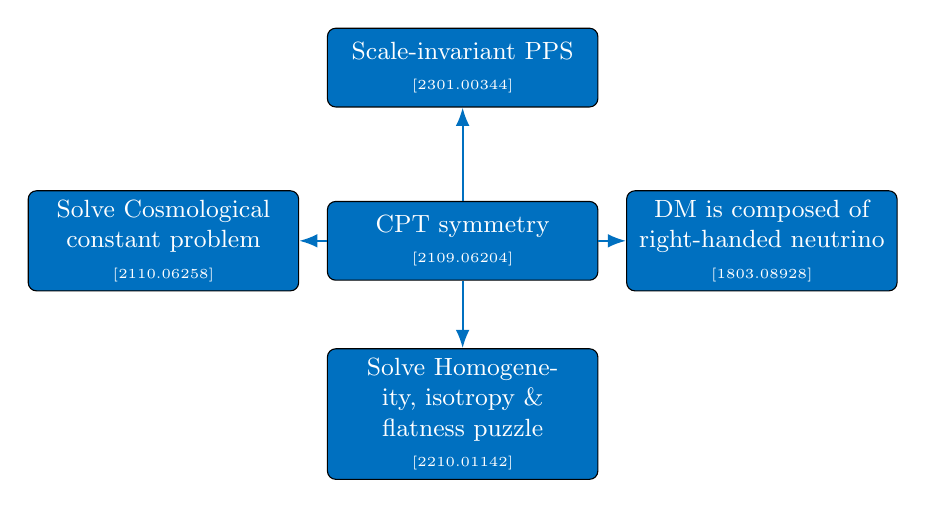
\begin{tikzpicture}[
      box/.style={draw, fill=cptblue, text=white, rounded corners=3pt,
                  text width=3.2cm, align=center, minimum height=1.0cm,
                  font=\small},
      arr/.style={-Latex, thick, cptblue}
    ]
    \node[box] (cpt) at (0,0) {CPT symmetry \\ {\tiny [2109.06204]}};
    \node[box] (flat) at (0,-2.2) {Solve Homogeneity, isotropy \& flatness puzzle \\ {\tiny [2210.01142]}};
    \node[box] (cc)   at (-3.8,0) {Solve Cosmological constant problem \\ {\tiny [2110.06258]}};
    \node[box] (dm)   at ( 3.8,0) {DM is composed of right-handed neutrino \\ {\tiny [1803.08928]}};
    \node[box] (pps)  at (0, 2.2) {Scale-invariant PPS \\ {\tiny [2301.00344]}};

    \draw[arr] (cpt) -- (flat);
    \draw[arr] (cpt) -- (cc);
    \draw[arr] (cpt) -- (dm);
    \draw[arr] (cpt) -- (pps);
  \end{tikzpicture}

  \vspace{0.3em}
  \Red{\textbf{How about perturbations?}}
  \end{center}
\end{frame}

%%================================================================
%%  PART 2 -- Theoretical Prediction of Spatial Curvature
%%================================================================
\begin{frame}{Outline}
  Part 1: Introduction -- CPT-symmetric universe\\[0.5em]
  \textbf{\Blue{Part 2: Theoretical prediction of $\Omega_K$}}
  \small (PRD\,110,\,103528;\; PRD\,113,\,023546)\\[0.5em]
  Part 3: K\"{a}hler-Dirac fermions -- Physical foundation of CPT
  \small (arXiv:2511.11548)\\[0.5em]
  Future directions: Lattice KD,\; Composite Higgs,\; Quadratic gravity

  \vspace{0.4cm}
  \begin{columns}[c]
    \column{0.45\textwidth}\centering
      \includegraphics[height=3.8cm]{\figpath wh260.jpg}\\
      {\small Will Handley (University of Cambridge)\\
       \texttt{wh260@cam.ac.uk}}
    \column{0.45\textwidth}\centering
      \includegraphics[height=3.8cm]{\figpath lboyle3.jpg}\\
      {\small Latham Boyle (University of Edinburgh)\\
       \texttt{Latham.Boyle@ed.ac.uk}}
  \end{columns}
\end{frame}

%% ------------------------------------------------------------------
%%  P2-1  Resonant cavity analogy: CPT → antisymmetric perturbations
%% ------------------------------------------------------------------
\begin{frame}{Perturbations must be CPT-symmetric: the resonant cavity}
  \begin{columns}[c]
    \column{0.52\textwidth}
     Perturbations oscillate in conformal time $\Phi(k,\eta) \propto \cos\theta(k,\eta)$\\
      \textbf{Consequences for perturbations:}
      \begin{itemize}
        \item Perturbations must be \Blue{(anti-)symmetric}, otherwise would blow up at the future Big Bang (anti-universe). \small Lasenby et al.\ \arxiv{2104.02521}.
        \item This is the resonant cavity condition:
              only ``standing-wave'' modes are allowed
        \item Analogy: a resonant cavity selects discrete frequencies
      \end{itemize}
      \vspace{0.4em}
      \[
        \theta(k,\eta=\eta_\infty) = m\frac{\pi}{2},\quad m\in\mathbb{N}
      \]
      \Red{$\Rightarrow$ Only a \textbf{discrete set of $k$} is allowed.}
    \column{0.44\textwidth}
      \includegraphics[height=3cm,keepaspectratio]{\figpath CPT_periodic_FCB.png}\\[0.2em]
      \includegraphics[height=3.5cm,keepaspectratio]{\figpath standing_waves.png}\\
  \end{columns}
\end{frame}

%% ------------------------------------------------------------------
%%  P2-3  Spatial boundary condition in closed universe
%% ------------------------------------------------------------------
\begin{frame}{Spatial boundary condition in a closed universe}
  \begin{columns}[c]
    \column{0.52\textwidth}
      Closed universes have finite space
      $\Rightarrow$ an additional spatial boundary condition
      (in spherical harmonics)\\[0.5em]
      $\Rightarrow$ wave vectors have to be integers:
      \[
        k = n \in [1,2,3,\ldots]
      \]
      \vspace{0.3em}
      \Red{Matching the two discrete $k$ sets\\
           $\Rightarrow$ \textbf{constrains the curvature value.}}
    \column{0.44\textwidth}
      \includegraphics[width=\textwidth]{\figpath c0150405-closed_universe_artwork-spl-1.png}\\
      {\small Closed universe: finite spacetime volume}
  \end{columns}
\end{frame}

%% ------------------------------------------------------------------
%%  P2-4  Curvature controls spacing: the key idea
%% ------------------------------------------------------------------
\begin{frame}{Curvature controls the spacing -- matching the two discrete sets}
  \begin{columns}[c]
    \vspace{0.3em}
    \column{0.36\textwidth}
      Larger $|\Omega_K|$ $\rightarrow$ larger $\eta_\infty$\\[0.3em]
      Since $\Delta k \propto 1/\eta_\infty$,
      larger curvature means \textbf{smaller $\Delta k$}.\\[0.4em]
      \includegraphics[width=\textwidth]{\figpath loga-OmegaK.png}\\
      {\scriptsize $\Omega_{\kappa,0}$ more negative = universe lives longer}
    \column{0.6\textwidth}
      \Red{\textbf{Idea:}} Adjust $\Omega_K$ until the temporal discrete-$k$
      values become integers (required by the spatial BC).\\[0.3em]
      \movie[loop,autostart,width=\textwidth]{\includegraphics[width=\textwidth]{\figpath theta_kint_animation.png}}{\figpath theta_kint_animation.mp4}
  \end{columns}
\end{frame}

%% ------------------------------------------------------------------
%%  P2-5  Result: allowed Omega_K values and Planck observational status
%% ------------------------------------------------------------------
\begin{frame}{Result: predicted $\Omega_K$ and observational status}
  \begin{columns}[T]
    \column{0.46\textwidth}
      \textbf{Result (toy model, radiation only):}
      \begin{itemize}\small
        \item The integer-$k$ condition selects discrete values of $\Omega_K < 0$.
        \item Allowed gradient diverges at
              $\Omega_{\kappa,0}\simeq -0.012$ (big crunch limit).
      \end{itemize}
      \vspace{0.4em}
      \begin{block}{\small Observational status \hfill {\scriptsize PRD\,110,\,103528}}
        \small
        \textbf{Planck 2018 + lensing:}\\
        $\Omega_K = -0.044^{+0.018}_{-0.015}$\\[0.2em]
        ($2\sigma$ preference for closed universe)\\[0.2em]
        \textbf{Handley reanalysis:}\\
        $\sim3\sigma$ Bayesian tension for $\Omega_K < 0$
      \end{block}
    \column{0.50\textwidth}
      \includegraphics[width=\textwidth]{\figpath dtheta_dk_OmegaK.png}\\
      {\small $\Delta k$ (spacing of allowed $k$) vs $\Omega_K$.}
  \end{columns}
\end{frame}


%% ------------------------------------------------------------------
%%  P2-2  Discrete k from temporal BC (formal)
%% ------------------------------------------------------------------
\begin{frame}{Solve Perturbations in real cosmology}

  \vspace{0.1em}
  First few allowed modes of Perturbations\\
  $\Phi(k,\eta) \propto \cos\theta(k,\eta)$, 
  $\Phi$: Newtonian potential,\;
  $V$: velocity,\;
  $\delta$: density perturbation
  \vspace{0.3em}
  \begin{columns}[c]
    \column{0.9\textwidth}
      \includegraphics[width=\textwidth]{\figpath perturbation_solutions_transMatrix_timeseries_s-a.pdf}
    % \column{0.48\textwidth}
    %   \includegraphics[width=\textwidth]{\figpath dtheta_dk_OmegaK.png}
  \end{columns}
\end{frame}

%% ------------------------------------------------------------------
%%  P2-6 triangle plot
%% ------------------------------------------------------------------
\begin{frame}{Result: Planck MCMC triangle plot (Real Cosmology)}
  \begin{columns}[c]
    \column{0.38\textwidth}
      \begin{itemize}\small
        \item Calculate $\Delta k\in\mathbb{N}$ numerically with radiation anisotropy and higher order Boltamann terms.
        \item Filter Planck MCMC data with the $\Delta k\in\mathbb{N}$ constraint.
        \item Need joint analysis to break the degeneracy.
      \end{itemize}
      \includegraphics[width=\textwidth]{\figpath Planck_omegak_vs_chi2.pdf}
    \column{0.58\textwidth}
      \includegraphics[width=\textwidth]{\figpath Planck_TrianglePlot_diffDeltaK.pdf}
  \end{columns}
\end{frame}

%%================================================================

%% ------------------------------------------------------------------
%%  P2-7  Low-k eigenmodes: mathematical consistency
%% ------------------------------------------------------------------
\begin{frame}{Low-$k$ eigenmodes: mathematical consistency}
  \begin{columns}[c]
    \column{0.52\textwidth}
      \begin{enumerate}
        \item Large $k$: allowed wave vectors equally spaced (handled).
        \item Low $k$: valid solutions must satisfy \emph{both}
              spatial \emph{and} temporal BCs simultaneously
              $\Rightarrow$ linear combination of both bases:
              \[
                \Phi(x,t) = \sum_{n} c_n\phi_n
                           = \sum_{m} \tilde{c}_m\tilde{\phi}_m
              \]
        \item Coefficients = eigenvectors of mixing matrix $M$
              with eigenvalue $=1$.
      \end{enumerate}
    \column{0.44\textwidth}
      \includegraphics[width=\textwidth]{\figpath eigenvalue_2d_N25_Nt500_T3.14_m1.50_cylinder1.png}\\
      {\small Eigenvalue $=1$ selects valid low-$k$ modes.}
  \end{columns}
\end{frame}

%%================================================================
%%  PART 3 -- Kähler-Dirac Fermions
%%================================================================
\begin{frame}{Outline}
  Part 1: Introduction -- CPT-symmetric universe\\[0.5em]
  Part 2: Theoretical prediction of spatial curvature
  \small (PRD\,110,\,103528;\; PRD\,113,\,023546)\\[0.5em]
  \textbf{\Blue{Part 3: K\"{a}hler-Dirac fermions -- Physical foundation of CPT}}
  \small (arXiv:2511.11548)\\[0.5em]
  Future directions: Lattice KD,\; Composite Higgs,\; Quadratic gravity

  \vspace{0.4cm}
  \begin{columns}[c]
    \column{0.45\textwidth}\centering
      \includegraphics[height=3.8cm]{\figpath wh260.jpg}\\
      {\small Will Handley (University of Cambridge)\\
       \texttt{wh260@cam.ac.uk}}
    \column{0.45\textwidth}\centering
      \includegraphics[height=3.8cm]{\figpath lboyle3.jpg}\\
      {\small Latham Boyle (University of Edinburgh)\\
       \texttt{Latham.Boyle@ed.ac.uk}}
  \end{columns}
\end{frame}

%% ------------------------------------------------------------------
%%  P3-1  Problem: fermion doubling on the lattice
%% ------------------------------------------------------------------
\begin{frame}{Fermion doubling problem on the lattice}
  \begin{columns}[c]
    \column{0.52\textwidth}
      \textbf{Wilson's lattice gauge theory} works beautifully for bosons:
      \begin{itemize}
        \item 0-forms (scalars) $\to$ vertices
        \item 1-forms (gauge fields) $\to$ links
        \item 2-forms (field strengths) $\to$ plaquettes
      \end{itemize}
      \vspace{0.5em}
      \textbf{Problem with spinors:} no natural $p$-form interpretation
      $\Rightarrow$ placed on vertices $\Rightarrow$ \Red{extra doublers in the continuum limit}\\[0.4em]
      Chiral theory $\xrightarrow{\text{lattice}}$ non-chiral theory
      \hfill {\small (Nielsen--Ninomiya, 1981)}
    \column{0.44\textwidth}
      \includegraphics[width=\textwidth]{\figpath lattice.png}
  \end{columns}
\end{frame}

%% ------------------------------------------------------------------
%%  P3-2  Kähler-Dirac fermions
%% ------------------------------------------------------------------
\begin{frame}{K\"{a}hler-Dirac (KD) fermions}
  \textbf{Key idea:} KD fermions are $p$-forms -- they live naturally on any cell complex.

  \vspace{0.5em}
  \textbf{KD field} $\Phi$ is a \emph{polyform}: sum of $p$-forms ($p=0,\ldots,4$) with $16$ complex components.

  \vspace{0.4em}
  \textbf{KD action and equation:}
  \[
    S_{KD} = \langle\bar\Phi|(K-m)\Phi\rangle, \qquad
    (d - d^\dagger - m)\Phi = 0
  \]
  where $K = d - d^\dagger$,\quad $-K^2 = \square$ (wave operator on forms).

  \vspace{0.4em}
  Replacing $dx^\mu \to \gamma^\mu$ assembles the 16 components into a $4\times4$ matrix $\Psi$:
  \[
    (i\gamma^\mu\partial_\mu - m)\Psi = 0
    \quad\Rightarrow\quad
    S_{KD} = \int d^4x\;\mathrm{Tr}\!\left[\bar\Psi(i\slashed\partial - m)\Psi\right]
  \]
  with $\bar\Psi \equiv \gamma^0\Psi^\dagger\gamma^0$ (extra $\gamma^0$ on the left!).

  \vspace{0.3em}
  \textbf{Symmetry:} $\Psi'=U_{\Lambda} \Psi V, $ where $(U_{\Lambda}, V)\in \text{Spin}(3,1)\times U(2,2)$. 
  When restrict $V=U_{\Lambda}^{-1} \in SU(2,2)$, behave like forms.
\end{frame}

%% ------------------------------------------------------------------
%%  P3-3  The wrong-sign problem
%% ------------------------------------------------------------------
\begin{frame}{The wrong-sign problem in Lorentzian signature}
  Diagonalise the extra $\gamma^0$: $\gamma^0 = \Omega\Lambda\Omega^T$,
  $\Lambda = \mathrm{diag}(+1,+1,-1,-1)$.\\[0.5em]
  In terms of $\Psi' \equiv \Psi\Omega$:
  \[
    S_{KD} = \int d^4x\;\mathrm{Tr}\!\left[\Lambda\,\Psi'{}^\dagger\gamma^0
             (i\slashed\partial - m)\Psi'\right]
  \]
  \begin{itemize}
    \item Columns 1--2 of $\Psi'$: \Green{right sign} $\Rightarrow$ positive norm
    \item Columns 3--4 of $\Psi'$: \Red{wrong sign} $\Rightarrow$ \Red{negative norm states (ghosts)!}
  \end{itemize}

  \vspace{0.5em}
  \textbf{Resolution} (Donoghue \& Menezes) : a wrong-sign action = reversal of causality arrow
  $=$ \Blue{$PT$ reversal} \small [1908.04170].

  \vspace{0.4em}
  $\Rightarrow$ the two pairs of columns live on \textbf{two sheets} of spacetime, related by $PT$ symmetry
  (or, equivalently, $i \leftrightarrow -i$).
\end{frame}

% %% ------------------------------------------------------------------
% %%  P3-3b [NEW]  Connection to PT-symmetric field theories
% %% ------------------------------------------------------------------
% \begin{frame}{Connection to $PT$-symmetric field theories}
%   The KD wrong-sign problem is resolved via $PT$ reversal (Donoghue \& Menezes).\\[0.3em]
%   This is structurally parallel to a broader theme in non-Hermitian QFT:
%   \hfill{\small Alexandre, Bender et al.}

%   \vspace{0.3em}
%   \begin{columns}[T]
%     \column{0.48\textwidth}
%       \begin{block}{$PT$-symmetric QFT \hfill{\scriptsize Alexandre et al.}}
%         \begin{itemize}\small
%           \item Non-Hermitian Hamiltonians with $\mathcal{PT}$ symmetry
%                 can have \emph{real} spectra
%           \item A wrong-sign mass term becomes physical under $PT$ reversal
%           \item Dynamical mass generation via $\mathcal{PT}$ symmetry breaking
%         \end{itemize}
%       \end{block}
%     \column{0.48\textwidth}
%       \begin{block}{KD wrong-sign columns}
%         \begin{itemize}\small
%           \item Columns 3--4 of $\Psi'$ carry wrong-sign action
%           \item Wrong sign $=$ $PT$ reversal of the causal arrow
%           \item Both frameworks: a doubled structure resolves
%                 an apparently pathological sign problem
%         \end{itemize}
%       \end{block}
%   \end{columns}

%   \vspace{0.4em}
%   \Blue{Open question:} Is the KD-Majorana condition related to $\mathcal{PT}$-symmetric
%   mass generation on the two sheets?
%   Could the two-sheeted structure provide a \emph{geometric} realisation of
%   non-Hermitian field theory?
% \end{frame}

%% ------------------------------------------------------------------
%%  P3-4  Two-sheeted spacetime
%% ------------------------------------------------------------------
\begin{frame}{Two-sheeted spacetime}
  \begin{columns}[c]
    \column{0.6\textwidth}
      \begin{itemize}
        \item \Blue{Forward sheet} ($\Lambda_{ii}=+1$, cols 1--2):
              standard quantum mechanics with $e^{iS}$, $[x,p]=+i$
        \item \Blue{Backward sheet} ($\Lambda_{ii}=-1$, cols 3--4):
              uses $e^{-iS}$, $[x,p]=-i$
        \item The two sheets are \textbf{$PT$ mirrors} of each other
        \item Positive energy, positive norm on \emph{both} sheets
      \end{itemize}
      \vspace{0.5em}
      \textit{``Our" Big Bang is the junction of the two sheets --\\
      exactly the CPT-symmetric universe picture!}
    \column{0.4\textwidth}
      \includegraphics[width=\textwidth]{\figpath posi_neg_energy_waves2.png}\\[0.1em]
      \includegraphics[width=\textwidth]{\figpath CPT_periodic.png}
  \end{columns}
\end{frame}

%% ------------------------------------------------------------------
%%  P3-4b  Video: CPT mirror universe
%% ------------------------------------------------------------------
\begin{frame}{Physical explanation of the movie Tenet?}
  \begin{columns}[c]
    \column{0.75\textwidth}
  \begin{center}
    \movie[loop,autostart,width=\textwidth]{%
      \includegraphics[width=\textwidth]{\figpath tenet_movie_thumb.png}%
    }{\figpath tenet_movie_clip.mp4}
  \end{center}
    \column{0.25\textwidth}
    \includegraphics[width=\textwidth]{\figpath Tenet.png}
\end{columns}
\end{frame}

%% ------------------------------------------------------------------
%%  P3-5  KD-Majorana condition
%% ------------------------------------------------------------------
\begin{frame}{KD-Majorana condition}
  \textbf{Problem:} Two independent non-interacting sheets would double the particle content.

  \vspace{0.4em}
  \textbf{Solution:} Impose the \Blue{KD-Majorana condition}
  \[
    \Psi^c \equiv (i\gamma^2)\Psi^*(i\gamma^2) = \Psi
  \]
  In terms of $\Psi'$, the four columns are forced to take the form:
  \[
    \Psi' = \bigl(\psi_1,\;\psi_2,\;-\psi_2^c,\;\psi_1^c\bigr)
  \]

  \vspace{0.3em}
  \begin{columns}[c]
    \column{0.55\textwidth}
      \begin{itemize}
        \item A LH particle on the forward sheet is \emph{always} paired with
              a RH anti-particle on the backward sheet
        \item \Blue{Physical meaning:} CPT symmetry -- every particle has
              a mirror (anti-)partner on the other sheet
        \item No unphysical doubling of the SM
      \end{itemize}
    \column{0.42\textwidth}
      \includegraphics[width=\textwidth]{\figpath KD_Majorana.png}
  \end{columns}
\end{frame}

%% ------------------------------------------------------------------
%%  P3-6  Relation to the Standard Model
%% ------------------------------------------------------------------
\begin{frame}{Relation to the Standard Model}
  One SM generation (including $\nu_R$) = 16 Weyl spinors
  $=$ 4 KD-Majorana fields.\\[0.4em]
  Following Pati-Salam: allocate to four copies $\Psi'_{A=0,1,2,3}$ (\small [S. Catterall, 2209.03828])
  \[
    \Psi'_0 = \chi_0 + \chi_0^c,\quad
    \chi_0 = \begin{pmatrix}\nu_L & e_L \\ \nu_R & e_R\end{pmatrix}
    \quad\text{(leptons)}
  \]
  \[
    \Psi'_i = \chi_i + \chi_i^c,\quad
    \chi_i = \begin{pmatrix}u_L^i & d_L^i \\ u_R^i & d_R^i\end{pmatrix}
    \quad\text{(quarks, color }i=1,2,3)
  \]

  \vspace{0.3em}
  \textbf{Fermion kinetic terms unify:}
  \[
    \mathcal{L}_\text{KD} = \mathrm{Tr}\!\left[\bar\Psi_A(i\slashed\partial)\Psi_A\right],\quad A=0,\ldots,3
  \]
  Gauging $SU(3)\subset SU(4)$ and $SU(2)\times U(1)\subset U(2,2)$ (the internal symmetry)
  reproduces \emph{all} SM fermion kinetic terms.
\end{frame}

%% ------------------------------------------------------------------
%%  P3-7  Yukawa couplings unify
%% ------------------------------------------------------------------
\begin{frame}{Yukawa couplings unify in KD formalism}
  Standard Yukawa Lagrangian (4 separate terms):
  \[
    \tilde h^T\bar q_L u_R y_u + h^T\bar q_L d_R y_d
    + \tilde h^T\bar\ell_L \nu_R y_\nu + h^T\bar\ell_L e_R y_e
    + \text{h.c.}
  \]

  \vspace{0.3em}
  \textbf{KD formulation} (single compact expression):
  \[
    \mathcal{L}_Y = \mathrm{Tr}\!\left[
      \mathcal{H}^T\,\widehat\Psi_{A,L}^{\prime\,i}\,\Psi_{A,R}^{\prime\,j}\,
      \mathcal{Y}_A^{ij}
    \right] + \text{h.c.}
  \]
  where $\mathcal{H}$ is the \emph{KD Higgs field} and
  $\mathcal{Y}_A^{ij}$ the \emph{KD Yukawa matrix}.

  \vspace{0.4em}
  \begin{itemize}
    \item Expanding for leptons reproduces exactly the two lepton Yukawa terms
    \item Forward sheet $\leftrightarrow$ particles; backward sheet $\leftrightarrow$ antiparticles
    \item \Blue{All four SM Yukawa sectors unified in one line}
  \end{itemize}
\end{frame}

% %% ------------------------------------------------------------------
% %%  P3-8  Why must RH neutrinos exist? (KD explanation)
% %% ------------------------------------------------------------------
% \begin{frame}{Why must $\nu_R$'s exist? -- a new explanation}
%   \begin{columns}[c]
%     \column{0.55\textwidth}
%       \textbf{Old explanation:} seesaw mechanism explains small
%       $\nu_L$ masses.\\[0.5em]
%       \textbf{New (KD) explanation:}
%       \begin{itemize}
%         \item Each KD-Majorana field contains both LH \emph{and} RH components
%         \item Including $\nu_L$ in $\Psi'_0$ \emph{forces} the existence of $\nu_R$
%               on the same sheet
%         \item $\nu_R$ is \textbf{required by the geometry} of the KD field --
%               not just by phenomenology
%       \end{itemize}
%       \vspace{0.5em}
%       \Green{This is the new explanation promised at the start of the talk!}
%     \column{0.42\textwidth}
%       \includegraphics[width=\textwidth]{\figpath Seesaw_mechanism.png}
%   \end{columns}
% \end{frame}

%% ------------------------------------------------------------------
%%  P3-9  Connection to CPT-symmetric universe
%% ------------------------------------------------------------------
\begin{frame}{Connection to the CPT-symmetric universe}
  \begin{columns}[c]
    \column{0.68\textwidth}
      \textbf{Question:} \textit{Why} does the Big Bang act as a CPT mirror?\\[0.5em]
      The CPT-symmetric universe was motivated by observations
      (explain CMB and lots of cosmological phenomena).\\[0.4em]
      \textbf{KD answer:} Two sheeted is required for solving negative norm problem.
       The KD-Majorana condition \emph{requires} every particle
      to have a mirror (anti-)partner on the other sheet.\\[0.4em]
      \Blue{The Big Bang is precisely the junction where the two spacetime sheets meet.}
      \[
        \underbrace{\text{KD-Majorana}}_{\text{field theory}}
        \;\longleftrightarrow\;
        \underbrace{\text{CPT mirror at bang}}_{\text{cosmology}}
      \]
    \column{0.32\textwidth}
      \includegraphics[width=\textwidth]{\figpath CPT_periodic.png}
  \end{columns}
\end{frame}

%% ------------------------------------------------------------------
%%  P3-10  Black mirror (merged)
%% ------------------------------------------------------------------
\begin{frame}{Black mirror: an alternative black holes theory}
  \begin{columns}[c]
    \column{0.6\textwidth}
      \textbf{Standard picture:} black hole has an interior.\\[0.3em]
       \begin{itemize}\small
        \item Problem: Hidden from Observation? Curvature singularities? Information paradox?
         Violates all global symmetries (CPT, B-L)?
      \end{itemize}
      \textbf{Black mirror proposal} {\small [Tzanavaris, Latham \arxiv{2412.09558}]}
      \begin{itemize}\small
        \item The interior \emph{does not exist}
        \item The horizon mirrors our exterior to the
              ``other'' exterior (anti-universe)
        \item Infalling particles \emph{annihilate} with anti-partners
              from the anti-universe at the horizon
      \end{itemize}
      \vspace{0.em}
      \Green{KD-Majorana condition: explains why every infalling
      particle is paired with a mirror anti-partner.}
      \vspace{0.em}

      {\small\textit{Open question (for London): does the theory modify quasi-normal modes?}}
    \column{0.38\textwidth}
      \includegraphics[height=4.0cm,keepaspectratio]{\figpath Penrose_diagram_BHMirror.png}\\[0.2em]
      \includegraphics[height=2.6cm,keepaspectratio]{\figpath annihilate_BHmirror.png}
  \end{columns}
\end{frame}

%% ------------------------------------------------------------------
%%  P3-11  Theoretical description of Tenet
%% ------------------------------------------------------------------
\begin{frame}{Theoretical description of Tenet?!}
  \begin{columns}[T]
    \column{0.54\textwidth}
      \textbf{\Green{Same as CPT-symmetric universe:}}
      \begin{enumerate}
        \item There is \emph{you} and \emph{anti-you} in the universe
              and anti-universe
        \item Time goes backward in the anti-universe
        \item The doors connecting universe and anti-universe
              are \textbf{black holes}
      \end{enumerate}

      \vspace{0.5em}
      \textbf{\Red{Difference:}}
      \begin{enumerate}
        \item You and anti-you \textbf{annihilate} at the transition door
        \item If viewed from our universe: you come out of a
              \textbf{white hole} and find that time goes backward.
              However, you \emph{cannot change anything} -- only
              re-experience the past
      \end{enumerate}

    \column{0.43\textwidth}
      \includegraphics[width=\textwidth,keepaspectratio]{\figpath tenet_2.jpg}\\
      \includegraphics[width=\textwidth,keepaspectratio]{\figpath Periodic_BHMirror.png}
  \end{columns}
\end{frame}

%%================================================================
%%  FUTURE DIRECTIONS
%%================================================================
\begin{frame}{Outline}
  Part 1: Introduction -- CPT-symmetric universe\\[0.5em]
  Part 2: Theoretical prediction of spatial curvature
  \small (PRD\,110,\,103528;\; PRD\,113,\,023546)\\[0.5em]
  Part 3: K\"{a}hler-Dirac fermions -- Physical foundation of CPT
  \small (arXiv:2511.11548)\\[0.5em]
  \textbf{\Blue{Future directions: Lattice KD,\; Composite Higgs,\; Quadratic gravity}}

  \vspace{0.4cm}
  \begin{columns}[c]
    \column{0.45\textwidth}\centering
      \includegraphics[height=3.8cm]{\figpath wh260.jpg}\\
      {\small Will Handley (University of Cambridge)\\
       \texttt{wh260@cam.ac.uk}}
    \column{0.45\textwidth}\centering
      \includegraphics[height=3.8cm]{\figpath lboyle3.jpg}\\
      {\small Latham Boyle (University of Edinburgh)\\
       \texttt{Latham.Boyle@ed.ac.uk}}
  \end{columns}
\end{frame}

% ------------------------------------------------------------------
%  FD-1  KD on the lattice → chiral gauge theory
% ------------------------------------------------------------------
\begin{frame}[shrink=5]{Future direction 1: KD fermions on the lattice}
  {\footnotesize Boyle, Vaibhav (in preparation)}\\[0.1em]
  \begin{columns}[T]
    \column{0.8\textwidth}
      \textbf{\Red{Problem:} chirality in Euclidean signature}\\[0.1em]
      {\small KD operator $K$ anti-commutes with $\Gamma$
      $\Rightarrow$ Euclidean action $\langle\bar\Psi, K\Psi\rangle$
      mixes chiralities: \emph{cannot write a purely chiral action}}\\[0.2em]
      \textbf{\Blue{Solution:} mirror fermion space} {\footnotesize (Barrett \arxiv{2403.18428})}\\[0.1em]
      {\small Double the Hilbert space $\mathcal{H}'=\mathcal{H}\oplus\mathcal{H}$,
      with charge conjugation $J$ interchanging the two copies:}
        $S_{\rm chiral}=\tfrac{1}{2}\big< J'\Psi_L,K'\Psi_L\big>$\\[0.1em]
      \textbf{\Blue{'t~Hooft anomaly $\Rightarrow$ Pati-Salam}}\\[0.1em]
      {\small Cancelling the $\mathbb{Z}_4$ chiral anomaly on the lattice
      requires \textbf{4 copies} of reduced KD fermions
      $\Rightarrow$ gauge group $SU(4)\times SU(2)_L\times SU(2)_R$}\\[0.1em]
      \begin{block}{\small Two-sheeted spacetime is not just cosmology!}
        \small
        $\mathcal{H}'=\mathcal{H}\oplus\mathcal{H}$
        $\equiv$ universe $+$ anti-universe\\[0.1em]
        Required to simulate a \textbf{chiral gauge theory} on the lattice
        % (e.g.\ electroweak symmetry breaking, Pati-Salam unification)
      \end{block}
      \column{0.2\textwidth}
      \includegraphics[width=\textwidth]{\figpath lattice.png}\\[0.5em]
      {\footnotesize
        \textbf{Nielsen-Ninomiya} avoided:\\
        equal $n_L=n_R$ in Pati-Salam\\[0.4em]
        \textbf{Chiral anomaly} preserved\\
        on the lattice\\[0.4em]
        \textbf{Audience:} Alexandre, Sarkar}
  \end{columns}
\end{frame}


%% ------------------------------------------------------------------
%%  FD-2  Composite Higgs from dim-0 scalars
%% ------------------------------------------------------------------
\begin{frame}{Future direction 2: composite Higgs from dim-0 scalars}
  \begin{columns}[T]
    \column{0.58\textwidth}
      \textbf{Recall:} anomaly cancellation predicts
      $n_{s,1} = 0$ -- \emph{no fundamental dimension-1 scalars}.\\[0.3em]
      $\Rightarrow$ \textbf{The Higgs must be composite.}\\[0.4em]
      The challenge:
      \begin{itemize}
        \item Build a viable composite Higgs model from the
              collective dynamics of the \textbf{36 dim-0 scalar fields}
        \item Constrained by LHC data: no new physics at the TeV scale
              ($\kappa_V, \kappa_F$ within 5\% of SM)
        \item Must reproduce Higgs mass, couplings, and EW symmetry
              breaking without a fine-tuned hierarchy
      \end{itemize}
      \vspace{0.3em}
      \Green{Getting this right would unify the origin of cosmic
      structure and mass in a single framework.}
    \column{0.38\textwidth}
      \includegraphics[width=\textwidth]{\figpath SM_particles_dim0_RHnu.png}\\[0.2em]
      {\small \textbf{Audience:} Ellis, Tevong You (Higgs physics,
       SM EFT, composite Higgs)}
    \end{columns}
\end{frame}

%% ------------------------------------------------------------------
%%  FD-3  Quadratic gravity as architect of PPS
%% ------------------------------------------------------------------
\begin{frame}{Future direction 3: quadratic gravity as architect of the PPS}
  \begin{columns}[T]
    \column{\textwidth}
      \textbf{A deeper possibility:} the scale-invariant power
      spectrum may not require any new matter fields at all.\\[0.4em]
      \textbf{Quadratic gravity} (Stelle, 1977):
      \begin{itemize}
        \item Renormalizable theory of quantum gravity:\\
              $\mathcal{L} = \frac{2}{\kappa^2} R+ \frac{1}{6f_0^2} R^2 - \frac{1}{2\xi^2} C_{\mu\nu\alpha\beta}C^{\mu\nu\alpha\beta} $
        \item The ghost problem in quadratic gravity
              $\Rightarrow$ resolved by the Donoghue--Menezes
              $PT$ reversal \arxiv{2112.01974}.
        \item Initial results (Boyle): quadratic gravity at the
              Big Bang can \emph{mimic} the dim-0 scalar effect $\Rightarrow$ scale-invariant PPS without any new matter fields!
        \item Problem: need new explanation for cosmological constant problem.
      \end{itemize}
      \vspace{-1.5em}
      \begin{block}{}
        \small
        \textbf{Problem:} dim-0 scalars vs.\ quadratic gravity. Which one is the true architect of the scale-invariant PPS?
      \end{block}
      {\footnotesize \textbf{Audience:} Mavromatos, Sakellariadou, Lim,
       Gregory (quantum gravity, spectral geometry)}
  \end{columns}
\end{frame}

%% ------------------------------------------------------------------
%%  Summary
%% ------------------------------------------------------------------
\begin{frame}[shrink=15]{Summary}
  \begin{columns}[T]
    \column{0.50\textwidth}
      \textbf{Part 1: Introduction}
      \begin{itemize}\small
        \item CPT-symmetric universe solves flatness, CC, DM, PPS
        \item Extended SM: 3 $\nu_R$ + 36 dim-0 scalars; Higgs composite
        \item $\nu_R$ DM ($M\approx5\times10^8$ GeV); lightest $\nu$ massless
      \end{itemize}
      \textbf{Part 2: Quantized curvature}
      \begin{itemize}\small
        \item CPT $\Rightarrow$ perturbations must be (anti-)symmetric
        \item Temporal + spatial BCs $\Rightarrow$ discrete $k$
        \item Predicts $\Omega_K < 0$; $2\sigma$ Planck preference
      \end{itemize}
      \textbf{Future directions}
      \begin{itemize}\small
        \item KD on lattice $\Rightarrow$ chiral SM (lattice consistency)
        \item Composite Higgs from 36 dim-0 scalars (LHC test)
        \item Quadratic gravity as origin of scale-invariant PPS
      \end{itemize}
    \column{0.48\textwidth}
      \textbf{Part 3: K\"{a}hler-Dirac fermions}
      \hfill{\footnotesize arXiv:2511.11548}
      \begin{itemize}\small
        \item KD fermions = polyforms; live naturally on the lattice
        \item Wrong-sign columns $\Rightarrow$ two-sheeted spacetime
              ($PT$ mirrors; links to Alexandre et al.)
        \item KD-Majorana: every particle paired with mirror anti-partner
        \item Unifies all SM fermion kinetic + Yukawa terms
        \item \Blue{Explains \emph{why} the Big Bang is a CPT mirror}
        \item $\nu_R$ required by geometry
      \end{itemize}
      \vspace{0.2em}
      \centering
      \textbf{\Blue{Thank you!}}\\
      \small\texttt{wnd22@cam.ac.uk}\\
      \small\url{https://weiningdeng.com}
      \includegraphics[width=0.8\textwidth]{\figpath CPT-symmetric_universe.png}
  \end{columns}
\end{frame}

%%================================================================
%%  BACKUP SLIDES
%%================================================================
\appendix

%% ------------------------------------------------------------------
%%  P1-4 [NEW]  Two approaches to CPT at the quantum gravity interface
%% ------------------------------------------------------------------
\begin{frame}[noframenumbering]{Backup: Two approaches to CPT at the quantum gravity interface}
  \vspace{0.2em}
  {\small Both probe CPT in regimes where quantum gravity effects become relevant.}
  \vspace{0.4em}

  \begin{columns}[T]
    \column{0.48\textwidth}
      \begin{block}{\Blue{CPT-symmetric universe} \hfill {\scriptsize Boyle--Turok}}
        \begin{itemize}\small
          \item Universe + anti-universe pair, joined at the Big Bang
          \item CPT is an \textbf{exact} symmetry of the full spacetime
          \item Predictions: $\nu_R$ as DM, massless lightest $\nu$,
                scale-invariant PPS
        \end{itemize}
      \end{block}
    \column{0.48\textwidth}
      \begin{block}{\Blue{CPT violation from spacetime foam} \hfill {\scriptsize Mavromatos et al.}}
        \begin{itemize}\small
          \item Planck-scale foam induces \textbf{effective CPT violation}
          \item Quantum decoherence of propagating matter
          \item Predictions: modified EPR correlations in neutral
                mesons, neutrino anomalies
        \end{itemize}
      \end{block}
  \end{columns}

  \vspace{0.5em}
  \begin{center}
  \small
  \begin{tabular}{lccc}
    \toprule
    & CPT-symmetric universe & CPT foam & Standard inflation \\
    \midrule
    CPT status        & exact                   & violated & unspecified \\
    Quantum gravity & none     & considered     & depends (ex: string) \\
    DM candidate      & $\nu_R$                 & ---      & various (ex: axions)    \\
    Testable now?     & \Green{yes}             & \Green{yes} & \Green{yes} \\
    \bottomrule
  \end{tabular}
  \end{center}
\end{frame}

%% ------------------------------------------------------------------
%%  Backup: contour plot of Delta k
%% ------------------------------------------------------------------
\begin{frame}[noframenumbering]{Backup: contour plot of $\Delta k$}
  \begin{columns}[c]
    \column{0.40\textwidth}
      \[
        c(\Omega_K,\Omega_m,\Omega_b,h) = N \in \mathbb{N}
      \]
    \column{0.56\textwidth}
      \includegraphics[width=\textwidth]{\figpath DeltaK_contourPlot.png}
  \end{columns}
\end{frame}

%% ------------------------------------------------------------------
%%  Backup:  CMB power spectrum comparison
%% ------------------------------------------------------------------
\begin{frame}[noframenumbering]{Backup: CMB power spectrum comparison}
  \begin{columns}[c]
    \column{0.46\textwidth}
      Modify Boltzmann code CLASS to see how sparse wave vectors
      affect CMB power spectrum.
      \begin{enumerate}
        \item More fluctuations if $N$ and curvature ($\tilde{\kappa}$) become large.
        \item However, since $\Delta\tilde{k} = N\sqrt{\tilde{\kappa}}$,
              $N$ and $\tilde{\kappa}$ are negatively correlated
              $\rightarrow$ never both large.
        \item The fluctuation behaviour could be ignored.
      \end{enumerate}
    \column{0.50\textwidth}
      \includegraphics[width=\textwidth]{\figpath CMB_diff_nuspacing.pdf}
  \end{columns}
\end{frame}

\end{document}
